\nnarticleheader{Math Modeling Solution Paper Team 15201}{Gary Gao '21, Julius Huang '22, Elijah Lee '22, Adamya Aggarwal '22, Samuel Kohl '22}

\section*{Executive Summary}

	As technology develops, the impetus on governments and companies to provide widely accessible wifi solutions grows higher and higher; in many ways, your access to high-speed internet defines your lifestyle: in fact, many organizations, such as the U.N., define access to the internet as a human right. This reality has only been exacerbated by the COVID-19 pandemic- many students of disadvantaged socioeconomic backgrounds found themselves driving to parking lots and restaurants to learn virtually from a hotspot. Seeing this information, we are presented with the challenge of three problems: firstly, we have to predict pricing trends for different levels of bandwidth over the next ten years; secondly, we are asked to predict a family’s bandwidth needs based on certain characteristics; finally, we will develop a model optimally placing cell towers in three different regions, ensuring adequate coverage for all citizens based on their needs.\\
	\indent For the first problem, we used given and researched data to perform a multi-linear regression. This method will be further discussed later. We tested a couple of hypothetical factors that we think may affect the price of the Internet Plan and yield different results. \\
	\indent In the second problem, we used given data on age demographics and researched data to construct a rudimentary model on finding the bandwidth needs of a single family. This model takes into account age, employment, entertainment preferences.\\ 
	\indent For the third, we equated the given problem to the “maximal covering location problem” (MCLP). From there, we found our solution using the MCLP, and visualized it with a python simulation and data visualization. 

 
\section*{Mobilizing Mobile}
	\subsection*{Problem Redefined}
	Q3 asks us to find an optimal plan to place cell towers in a region and then demonstrate accuracy in the three hypothetical regions provided.
		
	\subsection*{Assumptions}
	\begin{itemize}
	\item Assumption 1: The word “optimal” in the problem means the most households get internet through the fewest cell towers.
	\item Assumption 2: As long as a house is within range of a tower, we consider it to be fully serviced in terms of bandwidth.
	\end{itemize}

	\subsection*{Approaching the Problem}
	We paralleled this problem to the Maximal Covering Location Problem (MCLP), whose objective is to minimize the number of facilities (that each have a fixed radius r that dictates its service area) necessary to cover the population of a set of n nodes.\\
	\indent Let’s define some variables before we begin.
	\begin{center} \begin{tabular} {|c|c|}
		\hline
		Variable & Definition \\
		\hline
		$g_i$ & Bandwidth demand of household i\\
		\hline
		$Y_i$ & Dummy variable representing whether household i is covered by a tower \\
		\hline
		$x_j$ & Dummy variable representing whether a cell tower is on/off (i.e. used or not) \\
		\hline
		$p$ & Budget constraint \\
		\hline
	\end{tabular} \end{center}
	\indent The MCLP can be modeled through a linear program as follows:
	\begin{center}
		Maximize $\sum_{i\in I} g_iY_i$ \\
		Subject to $\sum_{j\in J}x_j \geq Y_i$ and $\sum_{j\in J}x_j \geq p$ \\
		$x_j \in \{0,1\}, Y_i \in \{0,1\}$
	\end{center}
	Basically, we want to maximize the demand (or the number of households covered). A household cannot be covered unless a tower is turned on/used, and we want to fit the number of towers within a constrained budget. Remember, Yi = 1 if household i is covered by at least one facility, and 0 otherwise.

	\subsection*{Applying the MCLP to an Example}
	For an example simulation, we will be using a very simple service area, composed of one region that has 500 nodes (households) in blue. Each household requires a bandwidth of 20 Mbps and each tower can service an unlimited amount of bandwidth and can service at a range of 45 miles. The number of towers ($p$) was capped at 20, and in this random distribution model, the towers served the maximum number of households (56.8\% of the population), as seen in the image below:

\renewcommand{\thefigure}{1}
    \begin{figure}[!htb]
   \begin{minipage}{0.48\textwidth}
     \centering
     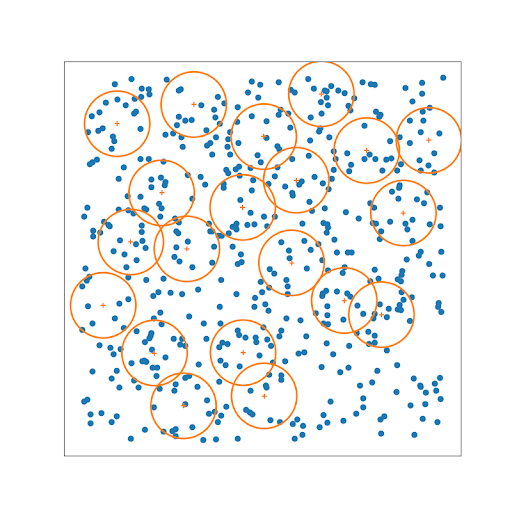
\includegraphics[width=.9\linewidth]{pic1.png}
     
   \end{minipage}\hfill
   \begin{minipage}{0.48\textwidth}
     \centering
     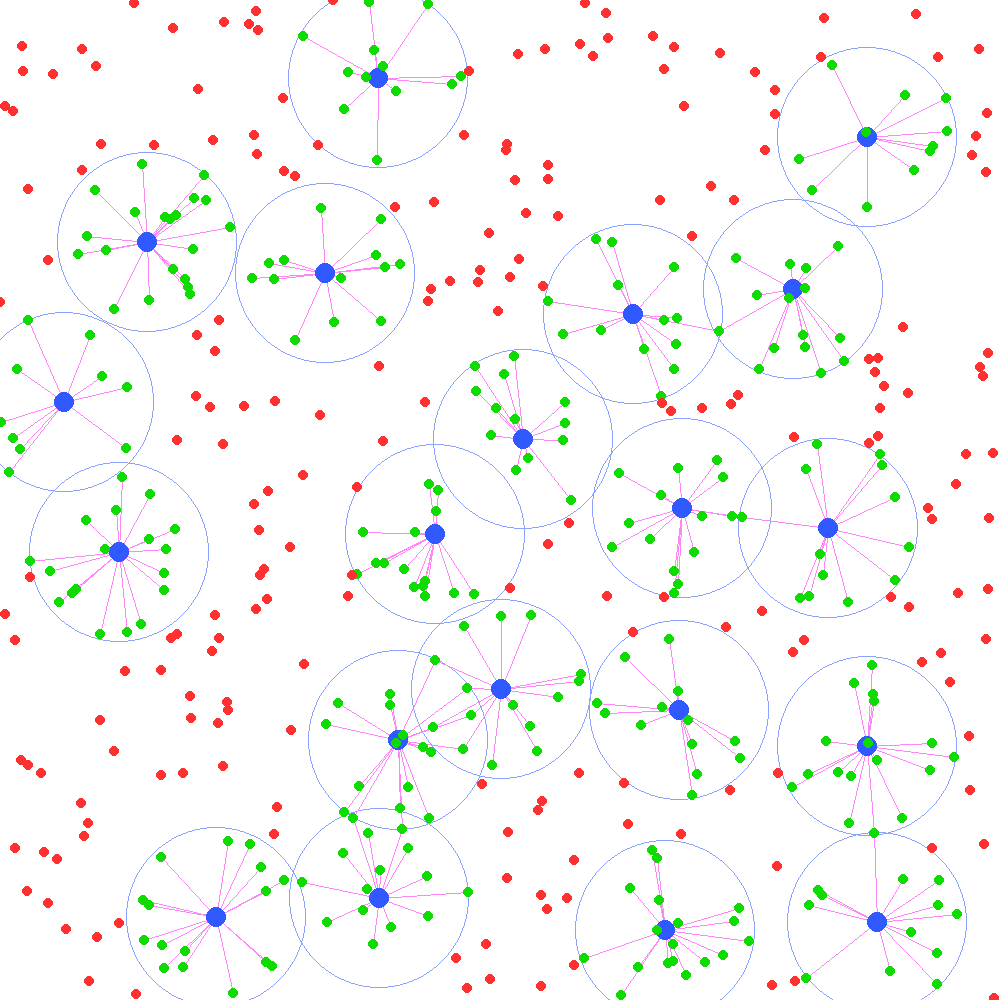
\includegraphics[width=.9\linewidth]{pic2.png}
     
   \end{minipage}
\end{figure}
    
    
    In the below image, we see a representation of the same scenario but with 40 stations, 45 range, 50mbps per household, and 650mbps throughput.
    
    \renewcommand{\thefigure}{1}
    \begin{figure}[!htb]
   \begin{minipage}{0.48\textwidth}
     \centering
     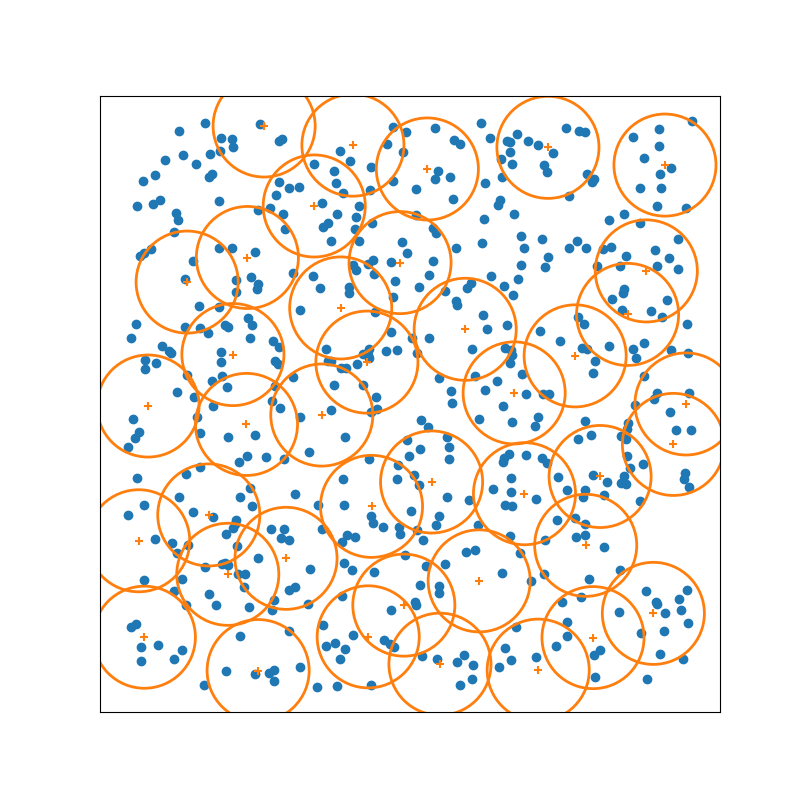
\includegraphics[width=.9\linewidth]{pic3.png}
     
   \end{minipage}\hfill
   \begin{minipage}{0.48\textwidth}
     \centering
     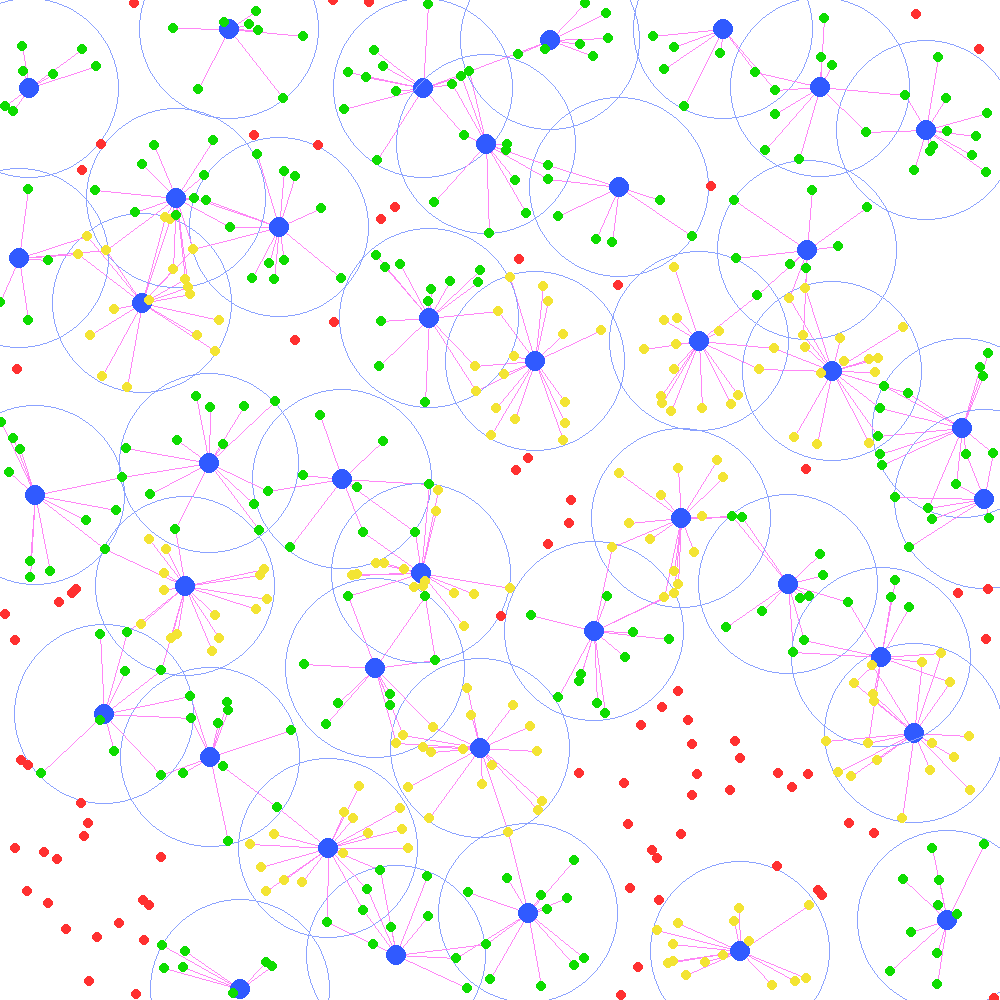
\includegraphics[width=.9\linewidth]{pic4.png}
     
   \end{minipage}
\end{figure}
    

	\subsection*{Simulation Algorithm}
	We created a simulation algorithm to visually represent households that are and aren't covered by a cell tower. Below is the skeleton of the algorithm in pseudocode.
	\begin{enumerate}
	\item For each node i, assign i to a tower if that tower’s range covers that node (note that one node can be assigned to multiple towers).
	\item Add its demand to a variable that represents the tower’s capacity. If a node is covered by two different towers, split its demand evenly and add the halved demand to each tower’s capacity.
	\item Any unserved nodes will be marked red.
	\item Iterate through the towers. If the sum of the demands of each node covered by a certain tower outweighs the tower’s capacity, assign each covered node the color yellow.
	\item Else, assign the nodes the color green.
	\end{enumerate}
	We can see the simulation algorithm results in the images below. In the first image, bandwidth per tower is capped at 200mbps total. 2\% of the nodes are green.
	\begin{figure}[h]
	\centering
	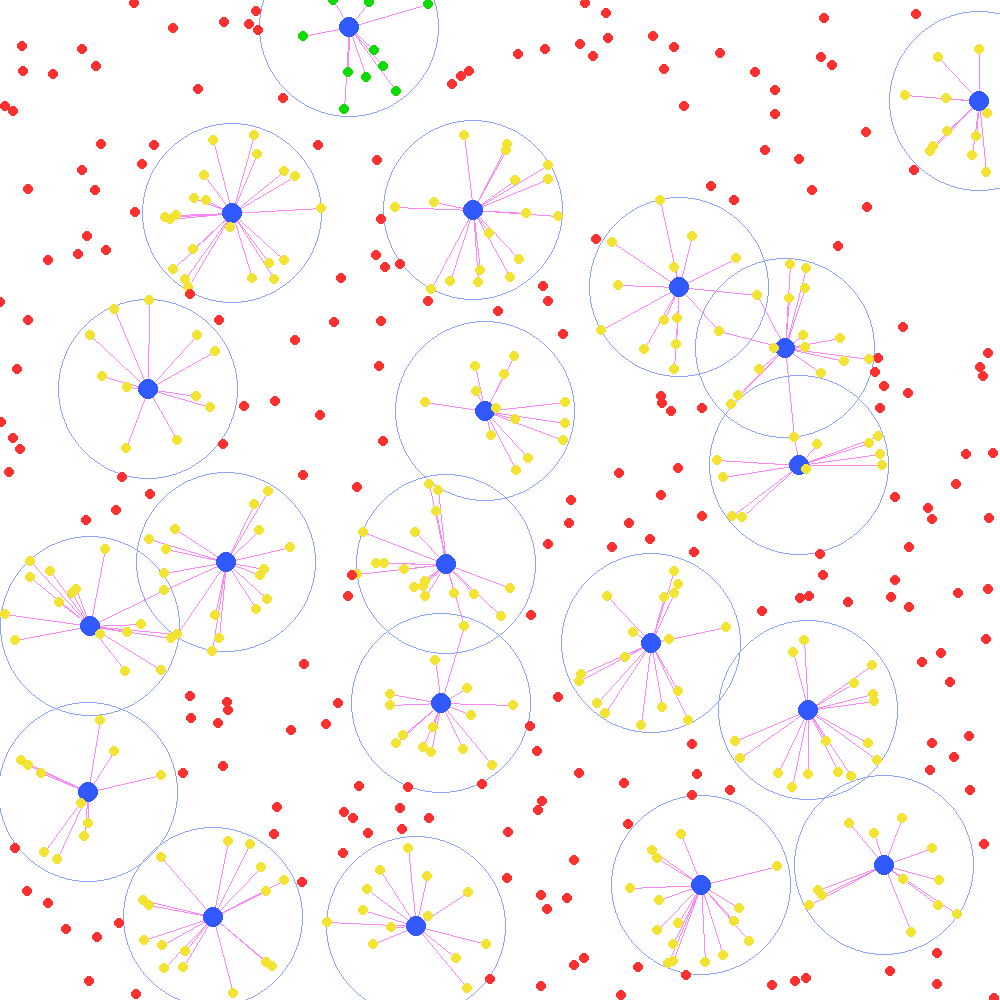
\includegraphics[width=0.5\linewidth]{pic5.png}
	\end{figure}
	
	\subsection*{Flaws and Additional Considerations for Improvements}
	\begin{itemize}
	\item Some houses may need to be in range of more than one tower to be fully serviced given the house’s bandwidth load.
	\item Some towers may be at full capacity and cannot provide bandwidth to any more households. We take this into account in our simulation software, which marks “fully loaded” towers yellow. However, our MCLP solver software does not take this into consideration.
	\item Using the MCLP may not be the most accurate because the solution to this problem, i.e. the minimum number of facilities required for total coverage, may exceed the affordable budget for infrastructure investment. If the budgetary constraint is incorporated in the model, then the objective would be to minimize the maximal service distance S.
	\end{itemize}
	
\section*{Appendix: Code}
	Simulation and MCLP Solver by Elijah Lee.\\
	\indent Note: MCLP solver adapted from https://github.com/cyang-kth/maximum-coverage-location\\
	\indent Note: run \verb|generate_random()| to generate a random distribution and save it for repeatability
	\begin{singlespace}
	\begin{verbatim}
import enum
import pygame
import math
from enum import Enum
 
import numpy as np
from scipy.spatial import distance_matrix
from gurobipy import *
from scipy.spatial import ConvexHull
from shapely.geometry import Polygon, Point
from numpy import random
import random
 
 
#######################################################
 
"""
 
Python implementation of the maximum coverage location problem.
 
The program randomly generates a set of candidate sites, among 
which the K optimal candidates are selected. The optimization 
problem is solved by integer programming. 
 
Author: Can Yang
Date: 2019-11-22
 
MIT License
 
Copyright (c) 2019 Can Yang
 
Permission is hereby granted, free of charge, to any person obtaining a copy
of this software and associated documentation files (the "Software"), to deal
in the Software without restriction, including without limitation the rights
to use, copy, modify, merge, publish, distribute, sublicense, and/or sell
copies of the Software, and to permit persons to whom the Software is
furnished to do so, subject to the following conditions:
 
The above copyright notice and this permission notice shall be included in all
copies or substantial portions of the Software.
 
THE SOFTWARE IS PROVIDED "AS IS", WITHOUT WARRANTY OF ANY KIND, EXPRESS OR
IMPLIED, INCLUDING BUT NOT LIMITED TO THE WARRANTIES OF MERCHANTABILITY,
FITNESS FOR A PARTICULAR PURPOSE AND NONINFRINGEMENT. IN NO EVENT SHALL THE
AUTHORS OR COPYRIGHT HOLDERS BE LIABLE FOR ANY CLAIM, DAMAGES OR OTHER
LIABILITY, WHETHER IN AN ACTION OF CONTRACT, TORT OR OTHERWISE, ARISING FROM,
OUT OF OR IN CONNECTION WITH THE SOFTWARE OR THE USE OR OTHER DEALINGS IN THE
SOFTWARE.
 
"""

def generate_candidate_sites(points,M=100):
    '''
    Generate M candidate sites with the convex hull of a point set
    Input:
        points: a Numpy array with shape of (N,2)
        M: the number of candidate sites to generate
    Return:
        sites: a Numpy array with shape of (M,2)
    '''
    hull = ConvexHull(points)
    polygon_points = points[hull.vertices]
    poly = Polygon(polygon_points)
    min_x, min_y, max_x, max_y = poly.bounds
    sites = []
    while len(sites) < M:
        random_point = Point([random.uniform(min_x, max_x),
                             random.uniform(min_y, max_y)])
        if (random_point.within(poly)):
            sites.append(random_point)
    return np.array([(p.x,p.y) for p in sites])
 
def mclp(points,K,radius,M):
    """
    Solve maximum covering location problem
    Input:
        points: input points, Numpy array in shape of [N,2]
        K: the number of sites to select
        radius: the radius of circle
        M: the number of candidate sites, which will randomly generated inside
        the ConvexHull wrapped by the polygon
    Return:
        opt_sites: locations K optimal sites, Numpy array in shape of [K,2]
        f: the optimal value of the objective function
    """
    print('----- Configurations -----')
    print('  Number of points %g' % points.shape[0])
    print('  K %g' % K)
    print('  Radius %g' % radius)
    print('  M %g' % M)
    import time
    start = time.time()
    sites = generate_candidate_sites(points,M)
    J = sites.shape[0]
    I = points.shape[0]
    D = distance_matrix(points,sites)
    mask1 = D<=radius
    D[mask1]=1
    D[~mask1]=0
    # Build model
    m = Model()
    # Add variables
    x = {}
    y = {}
    for i in range(I):
      y[i] = m.addVar(vtype=GRB.BINARY, name="y%d" % i)
    for j in range(J):
      x[j] = m.addVar(vtype=GRB.BINARY, name="x%d" % j)
 
    m.update()
    # Add constraints
    m.addConstr(quicksum(x[j] for j in range(J)) == K)
 
    for i in range(I):
        m.addConstr(quicksum(x[j] for j in np.where(D[i]==1)[0]) >= y[i])
 
    m.setObjective(quicksum(y[i]for i in range(I)),GRB.MAXIMIZE)
    m.setParam('OutputFlag', 0)
    m.optimize()
    end = time.time()
    print('----- Output -----')
    print('  Running time : %s seconds' % float(end-start))
    print('  Optimal coverage points: %g' % m.objVal)
    
    solution = []
    if m.status == GRB.Status.OPTIMAL:
        for v in m.getVars():
            # print v.varName,v.x
            if v.x==1 and v.varName[0]=="x":
               solution.append(int(v.varName[1:]))
    opt_sites = sites[solution]
    return opt_sites,m.objVal
 
def plot_input(points):
    '''
    Plot the result
    Input:
        points: input points, Numpy array in shape of [N,2]
        opt_sites: locations K optimal sites, Numpy array in shape of [K,2]
        radius: the radius of circle
    '''
    from matplotlib import pyplot as plt
    fig = plt.figure(figsize=(8,8))
    plt.scatter(points[:,0],points[:,1],c='C0')
    ax = plt.gca()
    ax.axis('equal')
   ax.tick_params(axis='both',left=False, top=False, right=False,
                       bottom=False, labelleft=False, labeltop=False,
                       labelright=False, labelbottom=False)
 
def plot_result(points,opt_sites,radius):
    '''
    Plot the result
    Input:
        points: input points, Numpy array in shape of [N,2]
        opt_sites: locations K optimal sites, Numpy array in shape of [K,2]
        radius: the radius of circle
    '''
    from matplotlib import pyplot as plt
    fig = plt.figure(figsize=(8,8))
    plt.scatter(points[:,0],points[:,1],c='C0')
    ax = plt.gca()
    plt.scatter(opt_sites[:,0],opt_sites[:,1],c='C1',marker='+')
    for site in opt_sites:
        circle = plt.Circle(site, radius, color='C1',fill=False,lw=2)
        ax.add_artist(circle)
    ax.axis('equal')
    ax.tick_params(axis='both',left=False, top=False, right=False,
                       bottom=False, labelleft=False, labeltop=False,
                       labelright=False, labelbottom=False)
    fig.show()
    input()
 
#######################################################
 
RESOLUTION = [1000, 1000]
PIXEL_MULTIPLIER = 2
 
TOWER_RANGE = 45
 
PINK = (255, 134, 246)
YELLOW = (243, 228, 51)
BLUE = (48, 90, 255)
RED = (255, 48, 48)
GREEN = (14, 220, 0)
LIGHT_BLUE = (139, 162, 255)
 
status_color = [RED, YELLOW, GREEN]
 
# keep track of marked nodes
visited = []
 
# Setup a class for each node
class Node:
    x = 0
    y = 0
    bandwidth = 0
 
    # for nodes, 0 = red (no service), 1 = orange (bandwidth issues), 2 = green (satisfied)
    # for towers, track demand
    status = -1
    
    def __init__(self, x, y, bandwidth, connection=None):
        self.x = x
        self.y = y
        self.bandwidth = bandwidth
        
        if connection == None:
            connection = []
        self.connection = connection
    
    def set_status(self, status):
        # do not update nodes marked yellow/red
        if self not in visited:
            self.status = status
            visited.append(self)
 
    def __str__(self):
        return "({}, {}) -- {}".format(self.x, self.y, self.bandwidth)
 
    def __repr__(self):
        return "({}, {}) -- {}".format(self.x, self.y, self.bandwidth)
 
nodes = []
towers = []
 
def reset_graph():
    for node in nodes:
        node.connection = []
    for tower in towers:
        tower.connection = []
 
# Connect nodes to their towers
def buildNodeGraph():
    reset_graph()
    for node in nodes:
        for tower in towers:
            if math.sqrt((node.x - tower.x)**2 + (node.y - tower.y)**2) <= TOWER_RANGE:
                tower.connection.append(node)
                node.connection.append(tower)
 
def calcNodeStatus():
    for node in nodes:
        if len(node.connection) == 0:
            node.set_status(0)
        elif len(node.connection) == 1:
            node.connection[0].status += node.bandwidth
        else:
            for tower in node.connection:
                tower.status += node.bandwidth / len(node.connection)
    
    for tower in towers:
        for node in tower.connection:
            node.set_status(1 if tower.status > tower.bandwidth else 2)
 
def score():
    green = 0
    for node in nodes:
        if node.status == 2:
            green += 1
    return green / len(nodes)
 
# Generate random point distribution
def generate_random():
    points = []
    # Region A, 500, 500 miles
    for i in range(0, 500):
        points.append(np.array([500 * random.random(), 500 * random.random()]))
    points = np.array(points)
    np.save("{}/profile.npy".format(os.path.dirname(os.path.abspath(__file__))), points)
 
# generate_random()
 
points = np.load("{}/profile.npy".format(os.path.dirname(os.path.abspath(__file__))))
 
# Starting number of sites to select
K = 40
 
# Service radius of each site
radius = 45
 
# Candidate site size (random sites generated)
M = 100
 
points = np.array(points)
 
# Run mclp 
# opt_sites is the location of optimal sites 
# f is the number of points covered
opt_sites,f = mclp(points,K,radius,M)
 
# Plot the result 
plot_result(points,opt_sites,radius)

 
for point in points:
    nodes.append(Node(point[0], point[1], 50))
for tower in opt_sites:
    towers.append(Node(tower[0], tower[1], 650))
 
# nodes = [Node(30, 20, 100), Node(20, 40, 50), Node(20, 55, 100)]
# towers = [Node(20, 30, 200), Node(20, 60, 200)]
 
buildNodeGraph()
calcNodeStatus()
 
print("SCORE: {}".format(score()))
 
# Initialize pygame
pygame.init()
screen = pygame.display.set_mode(RESOLUTION)
running = True
 
# Main loop
while running:
 
    # Event handling
    for event in pygame.event.get():
        if event.type == pygame.QUIT:
            running = False
 
    # Fill the background with white
    screen.fill((255, 255, 255))
 
    # Draw nodes
    for tower in towers:
    	for node in tower.connection:
    	pygame.draw.line(screen, PINK, (tower.x * PIXEL_MULTIPLIER, tower.y * PIXEL_MULTIPLIER), 
(node.x * PIXEL_MULTIPLIER, node.y * PIXEL_MULTIPLIER))
    pygame.draw.circle(screen, BLUE, (tower.x * PIXEL_MULTIPLIER, tower.y * PIXEL_MULTIPLIER), 10.0)
    pygame.draw.circle(screen, LIGHT_BLUE, (tower.x * PIXEL_MULTIPLIER, tower.y * 
PIXEL_MULTIPLIER), TOWER_RANGE * PIXEL_MULTIPLIER, 1)
    for node in nodes:
        pygame.draw.circle(screen, status_color[node.status], (node.x * PIXEL_MULTIPLIER, node.y 
* PIXEL_MULTIPLIER), 5.0)
    
    # Render
    pygame.display.flip()
 
pygame.quit()
 
	\end{verbatim}
	\end{singlespace}

\begin{thebibliography}{2}

\bibitem{} 
Measuring broadband america. (2021, February 12). Retrieved March 01, 2021, from https://www.fcc.gov/general/measuring-broadband-america

\bibitem{}
Markgraf, B. (2016, October 26). How far can a cell tower be for a cellphone to pick up the
signal? Retrieved March 02, 2021, from https://smallbusiness.chron.com/far-can-cell-
tower-cellphone-pick-up-signal-32124.html

\bibitem{}
Berry, J. J. (2020, August 27). COVID-19 exposes why access to the internet is a human
right. Retrieved March 02, 2021, from http://www.openglobalrights.org/covid-19-exposes-why-access-to-internet-is-human-right/.

\bibitem{}
Dvorak, Petula. “Perspective | When &#39;Back to School&#39; Means a Parking Lot and the Hunt for a
WiFi Signal.” The Washington Post, WP Company, 27 Aug. 2020,
www.washingtonpost.com/local/when-back-to-school-means-a-parking-lot-and-the-hunt-for-a-
wifi-signal/2020/08/27/0f785d5a-e873-11ea-970a-64c73a1c2392\_story.html.

\bibitem{}
Chung, C. (1986). Recent Applications of the Maximal Covering Location Planning
(M.C.L.P.) Model. Retrieved March 1, 2021, from https://www.jstor.org/stable/2581958

\bibitem{}
https://www.youtube.com/watch?v=i2Xy3VSkGRs

\bibitem{}
https://www.youtube.com/watch?v=sA8ItKmdwjM

\bibitem{}
Zarandi, M., Davari, S., &amp; Sisakht, S. (2011, November 19). The large scale maximal covering location problem. Retrieved March 02, 2021, from
https://www.sciencedirect.com/science/article/pii/S1026309811002100#s000040

\bibitem{} 
Snyder, S., &amp; Haight, R. (2016). Application of the Maximal Covering Location Problem
to Habitat Reserve Site Selection: A Review. Retrieved March 1, 2021, from
https://www.fs.fed.us/nrs/pubs/jrnl/2016/nrs\_2016\_snyder\_001.pdf

\bibitem{}
Goldstein, R. (2014, July 25). Duality in Linear Programming. Retrieved March 1, 2021,
from http://web.mit.edu/15.053/www/AMP-Chapter-04.pdf

\bibitem{}
Rodriguez, F., Blum, C., Lozano, M., &amp; Garcia-Martinez, C. (2012, April). Iterated Greedy
Algorithms for the Maximal Covering Location Problem. Retrieved March 1, 2021, from
https://www.researchgate.net/publication/265311031\_Iterated\_Greedy\_Algorithms\_for\_the\_Maximal\_Covering\_Location\_Problem


\end{thebibliography}
